\documentclass[a4paper]{article}

\usepackage{inputenc}
\usepackage[british,UKenglish]{babel}
\usepackage{amsmath}
%\usepackage{titlesec}
\usepackage{color}
\usepackage{graphicx}
\usepackage{fancyref}
\usepackage{hyperref}
\usepackage{float}
\usepackage{scrextend}
\usepackage{setspace}
\usepackage{xargs}
\usepackage{multicol}
\usepackage{nameref}

\usepackage{sectsty}
\usepackage{multicol}
\usepackage{multirow}
\usepackage[procnames]{listings}
\usepackage{appendix}

\newcommand\tab[1][1cm]{\hspace*{#1}}
\hypersetup{colorlinks=true, linkcolor=black}
\interfootnotelinepenalty=10000

\newcommand{\cleancode}[1]{\begin{addmargin}[3em]{3em}\texttt{\textcolor{cleanOrange}{#1}}\end{addmargin}}
\newcommand{\cleanstyle}[1]{\text{\textcolor{cleanOrange}{\texttt{#1}}}}


\usepackage[colorinlistoftodos,prependcaption,textsize=footnotesize]{todonotes}
\newcommandx{\commred}[2][1=]{\textcolor{Red}
{\todo[linecolor=red,backgroundcolor=red!25,bordercolor=red,#1]{#2}}}
\newcommandx{\commblue}[2][1=]{\textcolor{Blue}
{\todo[linecolor=blue,backgroundcolor=blue!25,bordercolor=blue,#1]{#2}}}
\newcommandx{\commgreen}[2][1=]{\textcolor{OliveGreen}{\todo[linecolor=OliveGreen,backgroundcolor=OliveGreen!25,bordercolor=OliveGreen,#1]{#2}}}
\newcommandx{\commpurp}[2][1=]{\textcolor{Plum}{\todo[linecolor=Plum,backgroundcolor=Plum!25,bordercolor=Plum,#1]{#2}}}

\def\code#1{{\tt #1}}

\def\note#1{\noindent{\bf [Note: #1]}}

\makeatletter
%% The "\@seccntformat" command is an auxiliary command
%% (see pp. 26f. of 'The LaTeX Companion,' 2nd. ed.)
\def\@seccntformat#1{\@ifundefined{#1@cntformat}%
   {\csname the#1\endcsname\quad}  % default
   {\csname #1@cntformat\endcsname}% enable individual control
}
\let\oldappendix\appendix %% save current definition of \appendix
\renewcommand\appendix{%
    \oldappendix
    \newcommand{\section@cntformat}{\appendixname~\thesection\quad}
}
\makeatother


% "define" Scala
\usepackage[T1]{fontenc}  
\usepackage[scaled=0.82]{beramono}  
\usepackage{microtype} 

\sbox0{\small\ttfamily A}
\edef\mybasewidth{\the\wd0 }

\lstdefinelanguage{scala}{
  morekeywords={abstract,case,catch,class,def,%
    do,else,extends,false,final,finally,%
    for,if,implicit,import,match,mixin,%
    new,null,object,override,package,%
    private,protected,requires,return,sealed,%
    super,this,throw,trait,true,try,%
    type,val,var,while,with,yield},
  sensitive=true,
  morecomment=[l]{//},
  morecomment=[n]{/*}{*/},
  morestring=[b]",
  morestring=[b]',
  morestring=[b]"""
}

\usepackage{color}
\definecolor{dkgreen}{rgb}{0,0.6,0}
\definecolor{gray}{rgb}{0.5,0.5,0.5}
\definecolor{mauve}{rgb}{0.58,0,0.82}

% Default settings for code listings
\lstset{frame=tb,
  language=scala,
  aboveskip=3mm,
  belowskip=3mm,
  showstringspaces=false,
  columns=fixed, % basewidth=\mybasewidth,
  basicstyle={\small\ttfamily},
  numbers=none,
  numberstyle=\footnotesize\color{gray},
  % identifierstyle=\color{red},
  keywordstyle=\color{blue},
  commentstyle=\color{dkgreen},
  stringstyle=\color{mauve},
  frame=single,
  breaklines=true,
  breakatwhitespace=true,
  procnamekeys={def, val, var, class, trait, object, extends},
  procnamestyle=\ttfamily\color{red},
  tabsize=2
}

\lstnewenvironment{scala}[1][]
{\lstset{language=scala,#1}}
{}
\lstnewenvironment{cpp}[1][]
{\lstset{language=C++,#1}}
{}
\lstnewenvironment{bash}[1][]
{\lstset{language=bash,#1}}
{}
\lstnewenvironment{verilog}[1][]
{\lstset{language=verilog,#1}}
{}



%代码段设置
\usepackage{listings}
\lstset{
breaklines,% 自动换行
basicstyle=\small,
escapeinside=,
keywordstyle=\color{ blue!70} \bfseries,
commentstyle=\color{red!50!green!50!blue!50},%
stringstyle=\ttfamily,%
extendedchars=false,%
linewidth=\textwidth,%
numbers=left,%
numberstyle=\tiny \color{blue!50},%
frame=trbl%
rulesepcolor= \color{ red!20!green!20!blue!20}
}

% 定义配色方案
\definecolor{codebg}{RGB}{245,245,244}      % 背景色（淡灰）
\definecolor{codegray}{RGB}{153,153,153}    % 行号/灰色
\definecolor{codegreen}{RGB}{0,128,0}       % 注释绿色
\definecolor{codeblue}{RGB}{0,102,204}      % 关键字蓝色
\definecolor{codepurple}{RGB}{163,21,21}    % 字符串棕红
\definecolor{codered}{RGB}{180,0,0}         % 错误/强调红

% 自定义样式
\lstdefinestyle{mystyle}{
    backgroundcolor=\color{codebg},         % 代码背景色
    commentstyle=\color{codegreen}\itshape, % 注释：绿色+斜体
    keywordstyle=\color{codeblue}\bfseries, % 关键字：蓝色+粗体
    numberstyle=\scriptsize\color{codegray},% 行号：灰色
    stringstyle=\color{codepurple},         % 字符串：紫红
    basicstyle=\ttfamily\small\linespread{1.1}\selectfont, % 基础：等宽+小号
    breakatwhitespace=false,
    breaklines=true,
    breakautoindent=true,
    captionpos=b,
    keepspaces=true,
    numbers=left,
    numbersep=8pt,
    showspaces=false,
    showstringspaces=false,
    showtabs=false,
    tabsize=4,
    frame=single,
    frameround=tttt,
    rulecolor=\color{black!20},
    escapeinside={\%*}{*)}
}

% 应用全局样式
\lstset{style=mystyle}

\graphicspath{ {images/} }
\usepackage[fontset=windows]{ctex} % 使用 Windows 系统中文字体（宋体/黑体/楷体/仿宋）
\usepackage{graphicx}
\usepackage{listings}
\usepackage{caption}
\usepackage{amssymb}
\usepackage{amsmath}
\usepackage{enumerate}
\usepackage{xcolor}
\usepackage{lastpage}%获得总页数
\usepackage{fancyhdr}
\usepackage{tabularx}
\usepackage{geometry}
\usepackage{cite}       % 参考文献数字引用
\usepackage{float}
\usepackage{multirow}
\usepackage{booktabs}
\usepackage{array}

%-------------------------页面边距--------------
\geometry{a4paper,left=2.3cm,right=2.3cm,top=2.7cm,bottom=2.7cm}
%-------------------------页眉页脚--------------
\pagestyle{fancy}
\fancyhf{}
\lhead{\kaishu 文本分类实现}
\rhead{\kaishu 自然语言处理实验报告}
\cfoot{\thepage}
\renewcommand{\headrulewidth}{0.1pt}
\renewcommand{\footrulewidth}{0pt}%去掉横线
\newcommand{\HRule}{\rule{\linewidth}{0.5mm}}%标题横线
\newcommand{\HRulegrossa}{\rule{\linewidth}{1.2mm}}
\setlength{\textfloatsep}{10mm}%设置图片的前后间距

% 命令行运行截图：可选参数为图片宽度，#1 图片文件名，#2 图题，#3 交叉引用标签
\newcommand{\runshot}[4][0.94\textwidth]{%
  \begin{figure}[H]
    \centering
    {\setlength{\fboxsep}{1pt}\setlength{\fboxrule}{0.5pt}%
     \fbox{\includegraphics[width={#1}]{#2}}}
    \caption{#3}\label{#4}
  \end{figure}}

%--------------------文档内容--------------------

\begin{document}
\renewcommand{\contentsname}{目\ 录}
\renewcommand{\appendixname}{附录}
\renewcommand{\appendixpagename}{附录}
\renewcommand{\refname}{参考文献}
\renewcommand{\figurename}{图}
\renewcommand{\tablename}{表}
\renewcommand{\today}{\number\year 年 \number\month 月 \number\day 日}

%-------------------------封面----------------
\begin{titlepage}
    \begin{center}
    
\includegraphics[width=0.8\textwidth]{NKU.png}\\[1cm]
    \vspace{16mm}
		\textbf{\huge\textbf{\kaishu{计算机学院}}}\\[0.5cm]
		\textbf{\huge{\kaishu{自然语言处理实验报告}}}\\[2.3cm]
		\textbf{\Huge\textbf{\kaishu{文本分类实现}}}

		\vspace{\fill}

    \centering
    {\Large\kaishu{姓\qquad 名\ :\ }\kaishu{余俊辉}}\\[0.55cm]
    {\Large\kaishu{学\qquad 号\ :\ }\kaishu{2313486}}\\[0.55cm]
    {\Large\kaishu{专\qquad 业\ :\ }\kaishu{计算机科学与技术}}

    \vfill
    {\Large \today}
    \end{center}
\end{titlepage}

\renewcommand {\thefigure}{\thesection{}.\arabic{figure}}%图片按章标号
\renewcommand{\figurename}{图}
\renewcommand{\tablename}{表}
\renewcommand{\contentsname}{目录}
\cfoot{\thepage\ /\ \pageref{LastPage}}%当前页/总页数

% 生成目录
\clearpage
\tableofcontents
\newpage

%==================================================================
\section{实验目的}
\label{sec:goal}

文本分类是自然语言处理中最基础也最典型的任务之一，它要求把一段文本映射到预先给定的类别。
同一份文本可以用完全不同的方式表示成计算机能够处理的向量，而表示方式的好坏往往直接决定了
分类器的上限。本次实验围绕 New York Times（NYT）新闻三分类任务，依次实现并比较三类
代表性的文本表示方法：基于词项统计的词袋模型（Bag-of-Words）、基于稠密词向量的平均文档表示
（Word2Vec / GloVe），以及对预训练语言模型 BERT 进行微调。三种方法共用同一份数据划分和同一套
评价指标，以便把差异归因于“表示方法”本身，而不是数据或评估口径的不同。

通过本次实验，希望达到以下目的：
\begin{enumerate}[(1)]
  \item 理解词袋、词向量与预训练语言模型这三类文本表示的基本思想与各自的适用场景；
  \item 走通“数据读取 $\rightarrow$ 划分与预处理 $\rightarrow$ 特征表示 $\rightarrow$ 训练分类器
        $\rightarrow$ 测试评估”这一完整的文本分类实验流程；
  \item 掌握 Logistic Regression 在高维文本特征上的使用方法；
  \item 掌握预训练 GloVe 的加载，以及使用 gensim 在外部语料上训练 Word2Vec 的方法；
  \item 熟悉使用 Hugging Face Transformers 对 BERT 进行文本分类微调的流程；
  \item 能够正确实现并解释 Accuracy 与 Macro-F1 两项指标，并据此对不同方法进行比较和分析。
\end{enumerate}

%==================================================================
\section{实验环境与数据集}
\label{sec:data}

\subsection{数据集介绍}
\label{sec:dataset}

实验使用两份数据，均为英文新闻文本：
\begin{itemize}
  \item \textbf{NYT 数据集}：主数据集，文件 \texttt{nyt.csv}，包含 \texttt{text}、\texttt{label}
        两列，共 11{,}519 条新闻，类别为 \texttt{sports}、\texttt{business}、\texttt{politics}
        三类。三个任务的模型都在该数据集上训练与评测。
  \item \textbf{AG News 数据集}：文件 \texttt{ag.csv}，仅含 \texttt{text} 一列，共 90{,}000 条新闻。
        本实验中它不参与分类训练，只作为额外语料，用于训练一组 Word2Vec 词向量。
\end{itemize}

NYT 的类别分布并不均衡，如表~\ref{tab:data} 所示，\texttt{sports} 一类就占了约四分之三，
另外两类各占约八分之一。这一特点会直接影响后面指标的选择（详见第~\ref{sec:metric} 节与
第~\ref{sec:analysis} 节的讨论）。

\begin{table}[H]
  \centering
  \caption{NYT 数据集的类别分布}
  \label{tab:data}
  \begin{tabular}{l r r r r}
    \toprule
    类别 & business & politics & sports & 合计 \\
    \midrule
    文档数量 & 1{,}429 & 1{,}451 & 8{,}639 & 11{,}519 \\
    占比     & 12.4\%  & 12.6\%  & 75.0\%  & 100\% \\
    \bottomrule
  \end{tabular}
\end{table}

\subsection{数据划分与预处理}
\label{sec:split}

按照作业要求，先对 NYT 做随机打乱，再按 $80\%/10\%/10\%$ 划分为训练集、验证集和测试集。
为了让结果可以复现，随机种子固定为 \texttt{RANDOM\_SEED=42}；同时采用\textbf{分层抽样}
（\texttt{stratify}），使三个集合中的类别比例与整体保持一致。具体做法是两次调用
\texttt{train\_test\_split}：先切出 10\% 作为测试集，再从剩余 90\% 中切出 $1/9$（即总量的 10\%）
作为验证集，剩下的 80\% 作为训练集，最终得到训练集 9{,}215 条、验证集 1{,}152 条、测试集
1{,}152 条，各集合的类别计数见表~\ref{tab:split}，对应分布见图~\ref{fig:classdist}。

\begin{table}[H]
  \centering
  \caption{固定随机种子（42）下的分层数据划分}
  \label{tab:split}
  \begin{tabular}{l c c c c}
    \toprule
    集合 & business & politics & sports & 合计 \\
    \midrule
    训练集 Train（80\%）       & 1{,}143 & 1{,}161 & 6{,}911 & 9{,}215 \\
    验证集 Validation（10\%）  & 143     & 145     & 864     & 1{,}152 \\
    测试集 Test（10\%）        & 143     & 145     & 864     & 1{,}152 \\
    \bottomrule
  \end{tabular}
\end{table}

\begin{figure}[htbp]
  \centering
  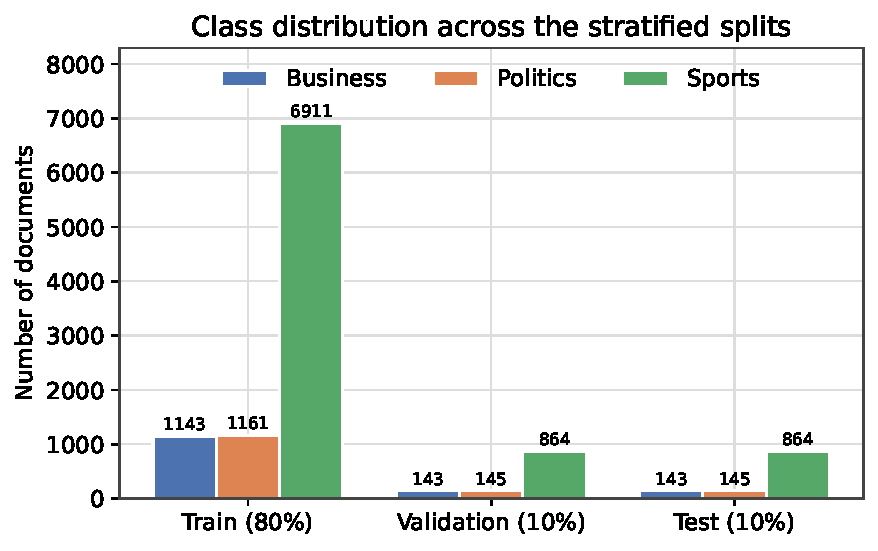
\includegraphics[width=0.78\textwidth]{fig_class_dist}
  \caption{分层划分后各集合的类别分布，三个集合的类别比例与整体基本一致}
  \label{fig:classdist}
\end{figure}

需要强调的是，\textbf{三个任务始终复用同一份划分}，最终性能统一在测试集（NYT Test Set）上报告，
保证六种实验设置之间的结果可以直接比较。

预处理方面，Task~1 和 Task~2 使用 NLTK\cite{bird2009nltk} 的 \texttt{word\_tokenize} 进行英文分词，并统一转为小写
（预训练 GloVe 词表本身为全小写，统一大小写可以减少未登录词，也保证各方法预处理口径一致）。
Task~3 不使用这一分词器，而是使用 BERT 自带的 WordPiece 子词分词器。为了避免数据泄漏，词袋的词表、
Word2Vec 词向量都只在\textbf{训练集}上学习，验证集和测试集只做相同的变换；在 NYT 上自训的
Word2Vec 也只使用训练集文本，而不接触验证集与测试集。

\subsection{实验环境}
\label{sec:env}

实验在一台配备 NVIDIA RTX 4060 Laptop（8\,GB 显存）的笔记本上完成，主要软件版本见表~\ref{tab:env}。
Task~1、Task~2 在 CPU 上即可快速完成；Task~3 在 GPU 上以半精度（fp16）微调，3 个 epoch
完整训练约 1 分 51 秒。

\begin{table}[H]
  \centering
  \caption{实验环境与主要依赖版本}
  \label{tab:env}
  \begin{tabular}{l l}
    \toprule
    项目 & 版本 / 说明 \\
    \midrule
    操作系统 & Windows（x64） \\
    Python   & 3.11 \\
    PyTorch  & 2.14.1（CUDA 12.6，GPU） \\
    Transformers & 5.19.0 \\
    Accelerate   & 1.15.0 \\
    scikit-learn & 1.9.1 \\
    gensim   & 4.4.0 \\
    NLTK     & 3.10.3 \\
    pandas / numpy & 3.0.6 / 2.4.6 \\
    预训练模型 & \texttt{google-bert/bert-base-uncased}、\texttt{glove.6B.100d} \\
    \bottomrule
  \end{tabular}
\end{table}

%==================================================================
\section{评价指标}
\label{sec:metric}

\textbf{准确率（Accuracy）}衡量分类正确的样本占全部样本的比例。设测试集共 $N$ 条样本，
第 $i$ 条的真实标签为 $y_i$、预测标签为 $\hat{y}_i$，则
\begin{equation}
  \mathrm{Accuracy} = \frac{1}{N}\sum_{i=1}^{N}\mathbb{1}\!\left(\hat{y}_i = y_i\right).
\end{equation}

\textbf{宏平均 F1（Macro-F1）}先逐个类别计算 F1，再对所有类别做无加权平均。对类别 $c$，
记真正例、假正例、假负例分别为 $\mathrm{TP}_c$、$\mathrm{FP}_c$、$\mathrm{FN}_c$，则
\begin{equation}
  P_c = \frac{\mathrm{TP}_c}{\mathrm{TP}_c+\mathrm{FP}_c}, \qquad
  R_c = \frac{\mathrm{TP}_c}{\mathrm{TP}_c+\mathrm{FN}_c}, \qquad
  F1_c = \frac{2P_cR_c}{P_c+R_c},
\end{equation}
\begin{equation}
  \mathrm{Macro\text{-}F1} = \frac{1}{C}\sum_{c=1}^{C} F1_c ,
\end{equation}
其中 $C$ 为类别数。若某个类别既没有真实样本也没有预测样本，约定其 F1 为 0
（与 scikit-learn 的 \texttt{zero\_division=0} 口径一致）。

在类别均衡时 Accuracy 直观且足够，但在本数据集这种大类（sports）占绝大多数的情况下，
即使模型对小类判得很差，Accuracy 仍然会显得很高。Macro-F1 对每个类别等权平均，不会被大类“带飞”，
因此更能反映模型在 business、politics 两个小类上的真实能力。本实验同时报告两项指标，
并以 Macro-F1 作为主要比较依据。

两项指标均在 \texttt{eval\_utils.py} 中手写实现。为了确认实现正确，本文将其结果与
scikit-learn 的 \texttt{accuracy\_score}、\texttt{f1\_score(average='macro')} 逐位对拍，
结果完全一致，包括某一类零预测的边界情形。

%==================================================================
\section{Task 1：词袋模型}
\label{sec:task1}

\subsection{方法原理}

词袋模型把文档看成一个无序的“词袋子”，忽略词序、句法和语法，只关心词表中的词在文档中
是否出现、出现多少次。设训练语料构建出的词表大小为 $|V|$，则每篇文档被表示为一个
$|V|$ 维的稀疏向量。

\textbf{Binary Bag of Words} 只记录词是否出现，向量第 $i$ 维为
\begin{equation}
  x_i =
  \begin{cases}
    1, & \text{若词表中第 } i \text{ 个词出现在该文档中},\\
    0, & \text{否则}.
  \end{cases}
\end{equation}

\textbf{Word Frequency（词频）}则记录出现次数，向量第 $i$ 维取该词在文档中的计数 $c_i$：
\begin{equation}
  \mathbf{x} = (c_1, c_2, \ldots, c_{|V|}).
\end{equation}
两者的区别在于：二值表示认为一个词出现一次和出现多次没有差别，词频表示则保留了这种强弱信息。

分类器统一使用 Logistic Regression。对 $K$ 分类问题，它对类别 $k$ 建模一个线性打分
$\mathbf{w}_k^\top\mathbf{x}+b_k$，再经 softmax 归一化为概率：
\begin{equation}
  p(y=k\mid\mathbf{x}) =
  \frac{\exp(\mathbf{w}_k^\top\mathbf{x}+b_k)}
       {\sum_{j=1}^{K}\exp(\mathbf{w}_j^\top\mathbf{x}+b_j)},
\end{equation}
训练时最大化带 $L_2$ 正则的对数似然（等价于最小化交叉熵损失加正则项）。
词袋特征维度高、极度稀疏，但不同类别往往由少量高度指示性的词线性决定，因此线性的
Logistic Regression 在这种特征上通常已经有很好的表现。

\subsection{实现细节}

直接使用 scikit-learn\cite{pedregosa2011scikit} 的 \texttt{CountVectorizer} 构建词袋，\texttt{analyzer} 指定为
项目统一的分词函数（其内部已完成小写化），通过 \texttt{binary} 开关在二值词袋与词频之间切换。
关键点在于\textbf{词表只在训练集上 \texttt{fit} 一次}，验证集、测试集仅做 \texttt{transform}，
杜绝测试集信息泄漏。本数据集构建出的词表规模为 127{,}018 维。核心代码如下：

\begin{lstlisting}[language=Python]
from sklearn.feature_extraction.text import CountVectorizer
from sklearn.linear_model import LogisticRegression

# fit on TRAIN only; binary=True -> Binary BoW, binary=False -> word frequency
vectorizer = CountVectorizer(analyzer=tokenize, binary=binary)
X_train = vectorizer.fit_transform(train_texts)
X_val   = vectorizer.transform(val_texts)
X_test  = vectorizer.transform(test_texts)

clf = LogisticRegression(max_iter=1000)
clf.fit(X_train, y_train)
y_pred = clf.predict(X_test)
\end{lstlisting}

\subsection{实验结果}

两种词袋表示在测试集上的结果见表~\ref{tab:res-task1}。两者的 Accuracy 相同（0.9826），
但词频表示的 Macro-F1 更高（0.9621 对 0.9576），说明“出现多少次”这一信息主要改善了
小类别的判别，这一点在 Accuracy 上看不出来，却被 Macro-F1 捕捉到了。

\begin{table}[H]
  \centering
  \caption{Task 1 在 NYT 测试集上的结果}
  \label{tab:res-task1}
  \begin{tabular}{l c c}
    \toprule
    表示方法 & Accuracy & Macro-F1 \\
    \midrule
    Binary Bag of Words + LR & 0.9826 & 0.9576 \\
    Word Frequency + LR      & 0.9826 & \textbf{0.9621} \\
    \bottomrule
  \end{tabular}
\end{table}

\runshot{shot_task1}{Task 1 词袋模型运行结果：终端打印两种词袋的矩阵形状与 Accuracy / Macro-F1}{fig:shot-task1}

%==================================================================
\section{Task 2：词向量表示}
\label{sec:task2}

\subsection{方法原理}

词袋向量维度高、稀疏，且任意两个维度之间相互独立，无法表达“近义词”这类语义关系。
词向量（word embedding）则把每个词映射为一个低维、稠密的实值向量，向量之间的距离和方向
能够编码语义相似性，其理论基础是分布式假设：\emph{出现在相似上下文中的词往往具有相似的含义}。

\textbf{Word2Vec}\cite{mikolov2013efficient,mikolov2013distributed} 是最具代表性的词向量学习方法之一，包含 CBOW 和 Skip-gram 两种结构。
本实验使用 gensim\cite{rehurek2010gensim} 默认的 CBOW：在一个上下文窗口内，用周围词的向量预测中心词，
训练完成后，网络的权重视为每个词的稠密向量。\textbf{GloVe}\cite{pennington2014glove} 则走另一条路线，它先基于全局
语料统计词与词的共现次数，再通过矩阵分解让词向量的点积拟合共现的对数加权值，从而同时利用
全局统计信息和局部上下文信息。

词向量是\emph{词级别}的表示，要得到\emph{文档级别}的特征，需要做一次聚合。按照作业要求，
对一篇包含 $n$ 个有效词的文档，取其词向量的平均作为文档向量：
\begin{equation}
  \mathbf{e}(d) = \frac{1}{n}\sum_{i=1}^{n}\mathbf{e}(w_i).
\end{equation}
实现时只对在词表中存在的词（有效词）求平均，未登录词（OOV）直接跳过；若整篇文档没有任何
有效词，则返回全零向量以避免除零。最后仍然用 Logistic Regression 在 100 维文档向量上分类。

\subsection{三组实验设置与实现}

三组实验使用完全相同的文档聚合与分类流程，区别只在于 100 维词向量的来源：
\begin{enumerate}[(1)]
  \item \textbf{预训练 GloVe}：加载 \texttt{glove.6B.100d}，该模型在约 60 亿 token 的通用
        语料上训练，词表约 40 万词。文件每行是“一个词 + 100 个数值”，逐行解析为
        “词 $\rightarrow$ 向量”的字典即可。
  \item \textbf{在 AG News 上自训 Word2Vec}：对 90{,}000 条 AG News 文本分词后训练
        CBOW 模型。
  \item \textbf{在 NYT 上自训 Word2Vec}：仅用 NYT \textbf{训练集}文本训练 CBOW 模型，
        以考察同领域语料的效果（同样不使用验证、测试集，防止泄漏）。
\end{enumerate}

两组自训 Word2Vec 的超参数保持一致：向量维度 100、上下文窗口 5、最低词频
\texttt{min\_count=5}、训练 5 个 epoch、固定随机种子 42。为了和 GloVe 统一接口，
训练好的 gensim 模型也导出为“词 $\rightarrow$ 向量”的字典，再走相同的文档平均与分类流程。
关键实现如下：

\begin{lstlisting}[language=Python]
from gensim.models import Word2Vec

# CBOW, 100-dim, window 5, drop words appearing fewer than 5 times
model = Word2Vec(sentences=sentences, vector_size=100, window=5,
                 min_count=5, workers=4, epochs=5, seed=42)
\end{lstlisting}

\begin{lstlisting}[language=Python]
import numpy as np

# average the embeddings of in-vocabulary words; OOV words are skipped
def doc_vector(tokens, embeddings):
    vectors = [embeddings[w] for w in tokens if w in embeddings]
    if len(vectors) == 0:
        return np.zeros(100, dtype=np.float32)   # all-OOV document
    return np.mean(np.stack(vectors), axis=0)
\end{lstlisting}

\subsection{实验结果}

三组词向量在测试集上的结果见表~\ref{tab:res-task2}。预训练 GloVe 最好，在规模更大的
AG News 上自训的 Word2Vec 次之，仅用 NYT 训练集自训的略低；三者整体都略低于 Task~1
的词袋模型。两组自训词向量之间的差距很小（Accuracy 仅相差 0.08 个百分点），具体原因
将在第~\ref{sec:analysis} 节统一分析。

\begin{table}[H]
  \centering
  \caption{Task 2 在 NYT 测试集上的结果}
  \label{tab:res-task2}
  \begin{tabular}{l c c}
    \toprule
    词向量来源 & Accuracy & Macro-F1 \\
    \midrule
    预训练 GloVe（glove.6B.100d）       & \textbf{0.9774} & \textbf{0.9468} \\
    Word2Vec，自训于 AG News（9 万篇）  & 0.9748 & 0.9406 \\
    Word2Vec，自训于 NYT 训练集（9 千篇）& 0.9740 & 0.9391 \\
    \bottomrule
  \end{tabular}
\end{table}

\runshot{shot_task2}{Task 2 词向量模型运行结果：终端依次打印 GloVe、AG-W2V、NYT-W2V 的特征矩阵形状与指标}{fig:shot-task2}

%==================================================================
\section{Task 3：BERT 微调}
\label{sec:task3}

\subsection{方法原理}

BERT（Bidirectional Encoder Representations from Transformers）建立在多层 Transformer
编码器之上\cite{vaswani2017attention}，核心是多头自注意力机制。与单向语言模型不同，BERT
通过掩码语言模型（MLM）和下一句预测（NSP）两个预训练任务，在大规模通用语料上学习到了
真正双向的上下文表示，同一个词在不同语境下会得到不同的向量，这从根本上区别于
Task~2 中“一个词只有一个固定向量”的静态词向量\cite{devlin2019bert}。

用于分类时，BERT 采用 WordPiece 子词分词，在序列首尾分别加上特殊标记 \texttt{[CLS]\_}
与 \texttt{[SEP]\_}，把 \texttt{[CLS]\_} 对应的最终隐状态接入一个线性分类头，输出各类别 logits。
预训练已经提供了很好的通用语言表示，因此下游任务通常只需要用标注数据对全部参数做少量轮次的
\textbf{微调（fine-tuning）}即可。

\subsection{实现细节}

使用 Hugging Face Transformers 实现\cite{wolf2020transformers}。代码优先加载随项目下载到本地的
\texttt{HW-1/bert-base-uncased}，目录缺失时再回退到在线仓库。分词时按作业要求设置
\texttt{max\_length=64}，超长截断、不足则填充到等长：

\begin{lstlisting}[language=Python]
from transformers import AutoTokenizer, AutoModelForSequenceClassification

tokenizer = AutoTokenizer.from_pretrained(MODEL_NAME)
encodings = tokenizer(list(texts),
                      truncation=True,
                      padding="max_length",
                      max_length=64)
model = AutoModelForSequenceClassification.from_pretrained(
    MODEL_NAME, num_labels=3, id2label=id2label, label2id=label2id)
\end{lstlisting}

训练通过 \texttt{Trainer} 完成，训练 3 个 epoch，训练批大小 16、评估批大小 32，
每个 epoch 在验证集上评估一次，GPU 可用时自动开启 fp16；评估回调复用本项目自己实现的
Accuracy 与 Macro-F1（对 logits 取 argmax 后计算）。

\begin{lstlisting}[language=Python]
training_args = TrainingArguments(
    output_dir="./results/bert",
    num_train_epochs=3,
    per_device_train_batch_size=16,
    per_device_eval_batch_size=32,
    eval_strategy="epoch",
    save_strategy="no",
    logging_steps=100,
    fp16=torch.cuda.is_available(),
    report_to=[])
trainer = Trainer(model=model, args=training_args,
                  train_dataset=train_ds, eval_dataset=val_ds,
                  processing_class=tokenizer, compute_metrics=compute_metrics)
trainer.train()
\end{lstlisting}

需要说明的是，加载预训练权重时终端会提示 \texttt{cls.predictions}、\texttt{cls.seq\_relationship}
等预训练头为“多余权重（UNEXPECTED）”，而 \texttt{classifier.weight/bias} 为“缺失权重
（MISSING）”。这是正常现象：前者是预训练阶段的 MLM/NSP 头，分类任务用不到；后者是下游
分类头，本就没有预训练权重、需要随机初始化后再微调。

\subsection{训练过程与结果}

训练共 1{,}728 个优化步，在 GPU 上以半精度训练耗时约 111 秒（1 分 51 秒）。验证集指标
随 epoch 的变化见表~\ref{tab:bert-epoch} 与图~\ref{fig:bertepoch}：第 2 个 epoch 达到峰值
（Accuracy 0.9809、Macro-F1 0.9599），第 3 个 epoch 略有回落；与此同时验证损失从第 1 个
epoch 的 0.0728 一路上升到第 3 个 epoch 的 0.0849，指标先升后降、损失却持续走高，是比较
典型的轻微过拟合迹象。最终在\textbf{测试集}上得到 Accuracy 0.9774、Macro-F1 0.9517。

\begin{table}[H]
  \centering
  \caption{BERT 各 epoch 验证集指标与最终测试集结果}
  \label{tab:bert-epoch}
  \begin{tabular}{l c c c}
    \toprule
    评估阶段 & 验证损失 & Accuracy & Macro-F1 \\
    \midrule
    验证集 Epoch 1 & 0.0728 & 0.9783 & 0.9527 \\
    验证集 Epoch 2 & 0.0823 & \textbf{0.9809} & \textbf{0.9599} \\
    验证集 Epoch 3 & 0.0849 & 0.9800 & 0.9545 \\
    \midrule
    \textbf{测试集（最终结果）} & --- & \textbf{0.9774} & \textbf{0.9517} \\
    \bottomrule
  \end{tabular}
\end{table}

\begin{figure}[htbp]
  \centering
  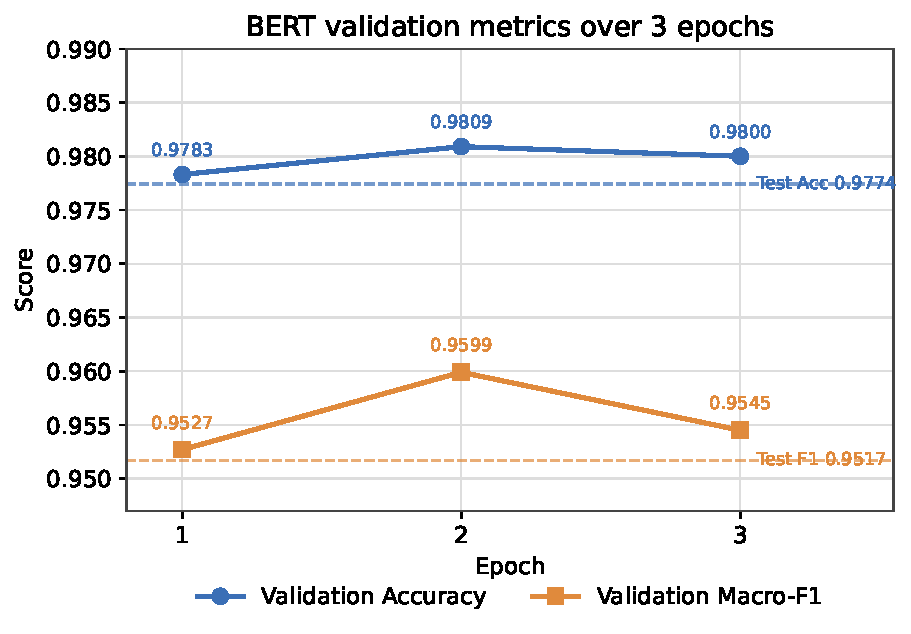
\includegraphics[width=0.82\textwidth]{fig_bert_epochs}
  \caption{BERT 三个 epoch 的验证集指标，虚线为最终测试集结果}
  \label{fig:bertepoch}
\end{figure}

\runshot[0.9\textwidth]{shot_task3}{Task 3 BERT 微调训练与测试结果：终端打印各 epoch 的训练/验证损失与指标，以及最终测试集 Accuracy / Macro-F1}{fig:shot-task3}

%==================================================================
\section{实验结果与分析}
\label{sec:analysis}

\subsection{总体结果}

六种实验设置在同一份测试集（1{,}152 条）上的结果汇总于表~\ref{tab:overall}，
对应的可视化对比如图~\ref{fig:resultsbar}。

\begin{table}[H]
  \centering
  \caption{六种实验设置在 NYT 测试集上的总体结果}
  \label{tab:overall}
  \begin{tabular}{l l c c}
    \toprule
    任务 & 方法 & Accuracy & Macro-F1 \\
    \midrule
    Task 1 & Binary BoW + LR            & \textbf{0.9826} & 0.9576 \\
    Task 1 & Word Frequency + LR        & \textbf{0.9826} & \textbf{0.9621} \\
    Task 2 & GloVe 平均向量 + LR        & 0.9774 & 0.9468 \\
    Task 2 & AG News 自训 Word2Vec + LR & 0.9748 & 0.9406 \\
    Task 2 & NYT 自训 Word2Vec + LR     & 0.9740 & 0.9391 \\
    Task 3 & BERT 微调                  & 0.9774 & 0.9517 \\
    \bottomrule
  \end{tabular}
\end{table}

\begin{figure}[htbp]
  \centering
  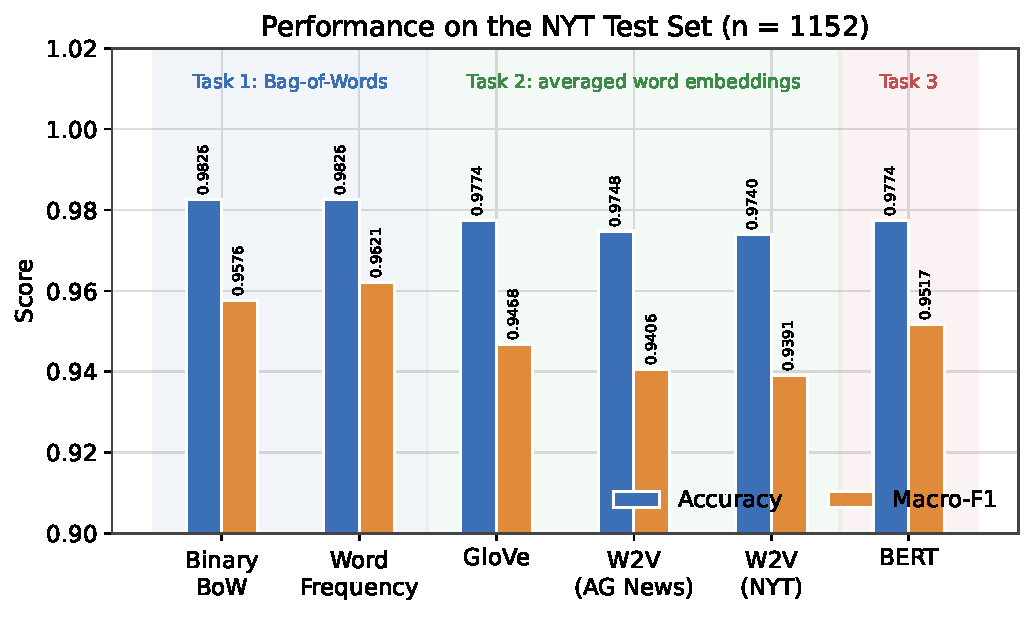
\includegraphics[width=0.95\textwidth]{fig_results_bar}
  \caption{六种实验设置在 NYT 测试集上的 Accuracy 与 Macro-F1 对比}
  \label{fig:resultsbar}
\end{figure}

\subsection{词袋为什么反超平均词向量}

从分数上看，最简单的词袋反而表现最好，Task~2 的平均词向量在 Accuracy 上落后约
0.5\,$\sim$\,0.9 个百分点，在 Macro-F1 上落后约 1.6\,$\sim$\,2.3 个百分点。
这并不矛盾，原因在于平均这一聚合方式损失了两类对主题分类至关重要的信息。
其一，\textbf{词频信息被抹平}：一个强指示词（如球队名、公司名、政治人物名）出现一次和
反复出现，在平均向量里几乎没有区别，而这正是词频词袋显式保留的。其二，\textbf{不同词的
贡献被相互抵消}：把成百上千个 100 维向量做算术平均后，文档被压缩成一个单一向量，
区分性词汇的信号被大量中性词稀释，词序信息也完全丢失。

相比之下，词袋保留了 127{,}018 维的细粒度词项特征。虽然维度很高，但特征稀疏、类别近似
线性可分，配合带 $L_2$ 正则的 Logistic Regression，恰好能稳定地从中学到每个指示词的权重。
换句话说，在“主题分类 + 指示词明确”这类任务上，高维稀疏的词袋并不是劣势，反而把最有用的
信息完整地留给了线性分类器。

\subsection{词向量来源：规模、覆盖与领域}

本次运行中 Task~2 内部的排序是 GloVe $>$ AG News 自训 $>$ NYT 自训，可以从语料规模、
词覆盖率和领域相关性三个角度解释。
\begin{itemize}
  \item \textbf{GloVe 明显最优}：它在约 60 亿 token 的通用语料上训练，词表约 40 万、
        覆盖率高，很多在 NYT 中出现次数很少、会被 \texttt{min\_count=5} 过滤掉的词，
        在 GloVe 中仍有向量，因此文档平均时有效词更多、表示更稳定，Accuracy 与 Macro-F1
        都明显领先两组自训词向量。
  \item \textbf{AG News 自训略优于 NYT 自训}：AG News 有 9 万篇，约为 NYT 训练集
        （9 千篇）的 10 倍，更大的语料让更多词满足 \texttt{min\_count=5}，词向量也训练得
        更充分，本次运行中以很小的优势（Accuracy 高 0.08、Macro-F1 高 0.15 个百分点）领先。
  \item 需要说明的是，两组自训词向量的这一差距非常小，落在神经网络训练随机性可能造成的
        数值波动范围之内，不宜据此断言“大规模跨领域语料一定优于同领域小语料”；本实验能
        稳妥得出的结论是：当语料规模相差约一个数量级时，规模与覆盖率的收益至少不弱于、
        甚至略超过领域匹配带来的收益。而无论哪一组自训词向量，受语料总量所限，覆盖率都
        远不及在 60 亿 token 上预训练的 GloVe。
\end{itemize}

\subsection{BERT 的表现与截断的影响}

BERT 的 Macro-F1 为 0.9517，高于 Task~2 中最好的平均词向量（GloVe 的 0.9468），
Accuracy 则与 GloVe 持平（均为 0.9774），说明上下文相关表示加微调在小类判别上确实强于
“静态向量 + 平均”。但它的两项指标都没有超过使用全文的词袋（Accuracy 0.9826、
Macro-F1 0.9621）。结合实验设置，本文认为主要有两点原因。

\textbf{第一，任务本身的上限。} NYT 三分类是典型的主题分类，类别由若干高度指示性的词汇
即可基本确定，词袋加线性分类器在这套数据上已经接近性能天花板，留给 BERT 的提升空间本就有限。

\textbf{第二，也是更关键的一点，输入长度被截断。} 作业要求 \texttt{max\_length=64}，
而 NYT 是完整的新闻文章。本文对全部文档按 NLTK 分词统计了长度，如图~\ref{fig:doclen}：
文档平均约 730 个词、中位数 768 词，最短 38 词、最长 5{,}977 词，\textbf{99.88\% 的文档
都超过了 64 个词}。考虑到 BERT 的 WordPiece 还会把一个词切成更细的子词，实际能容纳的
完整单词更少。也就是说，BERT 在三个任务里\emph{唯一}只看到了文章开头的一小段，正文绝大部分
内容都被丢弃；而 Task~1、Task~2 的特征是基于全文构建的。在这种信息不对等的情况下，
BERT 仍能在 Macro-F1 上超过全部平均词向量、在 Accuracy 上与最优的 GloVe 持平，
已经体现出预训练表示的能力。此外，验证集指标在第 2 个 epoch 见顶后回落、验证损失却从
0.0728 单调上升到 0.0849，说明在 9{,}215 条数据上对 1.1 亿参数的模型继续训练开始出现
轻微过拟合，3 个 epoch 已经足够。可以合理推测，若放宽最大长度（或对长文做分段、
滑动窗口等截断策略改进），让 BERT 看到更完整的文章，其性能应当能够超过词袋；
这一点可作为后续改进方向。

\begin{figure}[htbp]
  \centering
  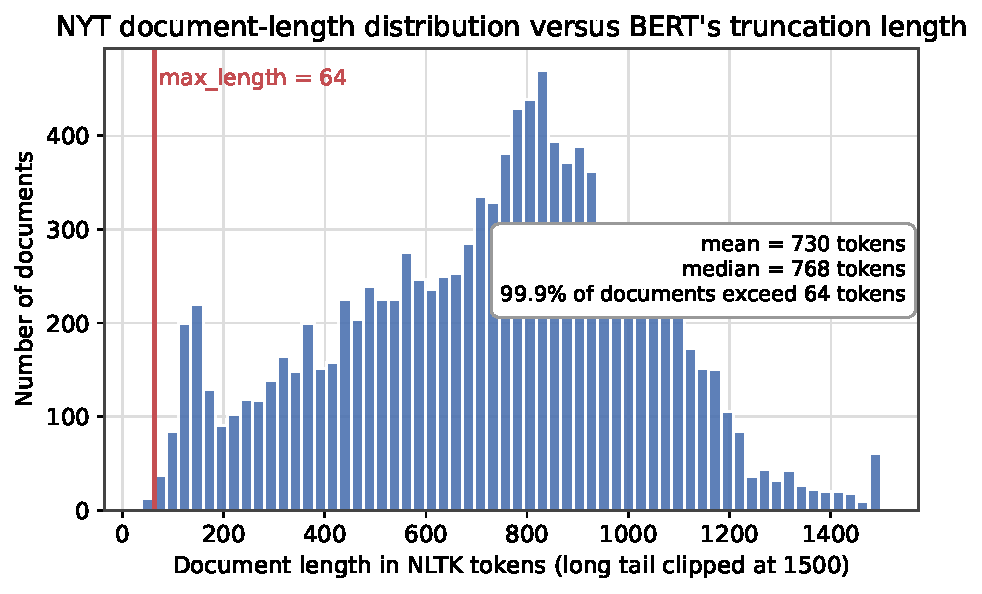
\includegraphics[width=0.92\textwidth]{fig_doc_length}
  \caption{NYT 文档长度分布与 BERT 截断长度（64）的对比，绝大多数文档远超该长度}
  \label{fig:doclen}
\end{figure}

\subsection{类别不均衡与指标选择}

由于 sports 占约 75\%，一个始终预测 sports 的平凡分类器也能拿到约 75\% 的 Accuracy，
这说明 Accuracy 在本任务上会被大类明显抬高。Macro-F1 对三个类别等权平均，business、politics
上的改善不会被 sports 掩盖。一个直接的例子是 Task~1：二值词袋与词频词袋的 Accuracy 完全相同
（0.9826），但 Macro-F1 相差 0.45 个百分点，差异正来自两个小类。这也印证了在不均衡数据集上
应当以 Macro-F1 为主、Accuracy 为辅来评价模型。

此外，本文通过固定随机种子保证了数据划分与 Word2Vec 训练的可复现性；不同硬件、不同库版本
可能带来合理范围内的微小数值波动，评价指标的手写实现也已与 scikit-learn 对拍一致，
因此上述横向比较是可靠的。

%==================================================================
\section{实验总结}
\label{sec:conclusion}

本次实验在同一份 NYT 数据、同一套划分和指标下，完整实现并比较了词袋、平均词向量和 BERT
三类文本表示。结果显示，文本分类的效果并不与模型复杂度简单地成正比：在主题明确、指示词清晰的
任务上，朴素的词频词袋配合 Logistic Regression 取得了最高的 Macro-F1（0.9621），
两种词袋也并列取得了最高的 Accuracy（0.9826）；预训练 GloVe 凭借大规模语料和高覆盖率，
在平均词向量方法中明显最好，两组自训词向量中，语料规模大约 10 倍的 AG News 略优于仅用
9 千篇 NYT 训练集的结果，说明在规模差距悬殊时覆盖率的收益并不弱于领域匹配；BERT 的
Macro-F1 高于全部平均词向量、Accuracy 与 GloVe 持平，但受限于 \texttt{max\_length=64}
对长文的截断，未能超过使用全文的词袋。

通过这组对比可以体会到，\textbf{选择文本表示时不能只看模型是否“先进”，还要看它与任务特点、
输入长度、数据规模和预处理方式是否匹配}。预训练语言模型能力很强，但它的实际表现同样会受到
输入截断、训练轮数等工程因素的制约；而看似简单的传统方法，在合适的条件下依然是很强的基线。
后续可以从放宽输入长度、改进长文聚合方式、按类别加权缓解不均衡等方向继续提升。

%==================================================================
\appendix
\section{代码结构与运行说明}
\label{sec:appendix}

\subsection{代码结构}

完整代码已托管在 GitHub：
\url{https://github.com/Biansss/NKU-NLP/tree/main/hw1}，主要文件见表~\ref{tab:files}。

\begin{table}[H]
  \centering
  \caption{项目文件说明}
  \label{tab:files}
  \begin{tabularx}{\textwidth}{l X}
    \toprule
    文件 & 说明 \\
    \midrule
    \texttt{data\_utils.py}    & 数据读取、固定种子的分层划分、NLTK 分词、标签映射 \\
    \texttt{eval\_utils.py}    & 手写 Accuracy 与 Macro-F1 \\
    \texttt{task1\_bow.py}     & Task 1：二值/词频词袋 + Logistic Regression \\
    \texttt{task2\_word2vec.py}& Task 2：GloVe / Word2Vec 平均文档向量 + LR \\
    \texttt{task3\_bert.py}    & Task 3：BERT 微调 \\
    \texttt{requirements.txt}  & 依赖清单 \\
    \texttt{README.md}         & 数据准备与运行说明 \\
    \bottomrule
  \end{tabularx}
\end{table}

\subsection{数据与模型准备}

体积较大的数据与预训练文件统一放在代码目录的 \texttt{HW-1/} 下（不纳入版本管理）：
\begin{itemize}
  \item \texttt{HW-1/nyt.csv}、\texttt{HW-1/ag.csv}；
  \item 从 \texttt{glove.6B.zip} 中解压出的 \texttt{glove.6B.100d.txt}（仅需 100 维这一份）；
  \item BERT 模型目录 \texttt{HW-1/bert-base-uncased/}；若该目录不存在，程序会自动从
        Hugging Face 下载 \texttt{google-bert/bert-base-uncased}。
\end{itemize}

\subsection{运行方式}

配置好环境并准备好数据后，依次运行三个脚本即可复现全部结果：

\begin{lstlisting}
conda activate nlp-hw1
python data_utils.py        # optional: check the split sizes
python task1_bow.py         # Task 1: Bag-of-Words
python task2_word2vec.py    # Task 2: GloVe / Word2Vec
python task3_bert.py        # Task 3: BERT fine-tuning
\end{lstlisting}

\runshot[0.9\textwidth]{shot_data}{数据读取与划分自检结果：终端打印 NYT 总条数、train/val/test 划分条数与分词示例}{fig:shot-data}

\bibliographystyle{plain}
\bibliography{reference}

\end{document}
